% Options for packages loaded elsewhere
\PassOptionsToPackage{unicode}{hyperref}
\PassOptionsToPackage{hyphens}{url}
%
\documentclass[
]{report}
\usepackage{lmodern}
\usepackage{amssymb,amsmath}
\usepackage{ifxetex,ifluatex}
\ifnum 0\ifxetex 1\fi\ifluatex 1\fi=0 % if pdftex
  \usepackage[T1]{fontenc}
  \usepackage[utf8]{inputenc}
  \usepackage{textcomp} % provide euro and other symbols
\else % if luatex or xetex
  \usepackage{unicode-math}
  \defaultfontfeatures{Scale=MatchLowercase}
  \defaultfontfeatures[\rmfamily]{Ligatures=TeX,Scale=1}
\fi
% Use upquote if available, for straight quotes in verbatim environments
\IfFileExists{upquote.sty}{\usepackage{upquote}}{}
\IfFileExists{microtype.sty}{% use microtype if available
  \usepackage[]{microtype}
  \UseMicrotypeSet[protrusion]{basicmath} % disable protrusion for tt fonts
}{}
\makeatletter
\@ifundefined{KOMAClassName}{% if non-KOMA class
  \IfFileExists{parskip.sty}{%
    \usepackage{parskip}
  }{% else
    \setlength{\parindent}{0pt}
    \setlength{\parskip}{6pt plus 2pt minus 1pt}}
}{% if KOMA class
  \KOMAoptions{parskip=half}}
\makeatother
\usepackage{xcolor}
\IfFileExists{xurl.sty}{\usepackage{xurl}}{} % add URL line breaks if available
\IfFileExists{bookmark.sty}{\usepackage{bookmark}}{\usepackage{hyperref}}
\hypersetup{
  pdftitle={  STAT 216 Activity Coursepack},
  pdfauthor={Melinda Yager, Jade Schmidt, Dr.~Stacey Hancock},
  hidelinks,
  pdfcreator={LaTeX via pandoc}}
\urlstyle{same} % disable monospaced font for URLs
\usepackage{longtable,booktabs}
% Correct order of tables after \paragraph or \subparagraph
\usepackage{etoolbox}
\makeatletter
\patchcmd\longtable{\par}{\if@noskipsec\mbox{}\fi\par}{}{}
\makeatother
% Allow footnotes in longtable head/foot
\IfFileExists{footnotehyper.sty}{\usepackage{footnotehyper}}{\usepackage{footnote}}
\makesavenoteenv{longtable}
\usepackage{graphicx}
\makeatletter
\def\maxwidth{\ifdim\Gin@nat@width>\linewidth\linewidth\else\Gin@nat@width\fi}
\def\maxheight{\ifdim\Gin@nat@height>\textheight\textheight\else\Gin@nat@height\fi}
\makeatother
% Scale images if necessary, so that they will not overflow the page
% margins by default, and it is still possible to overwrite the defaults
% using explicit options in \includegraphics[width, height, ...]{}
\setkeys{Gin}{width=\maxwidth,height=\maxheight,keepaspectratio}
% Set default figure placement to htbp
\makeatletter
\def\fps@figure{htbp}
\makeatother
\setlength{\emergencystretch}{3em} % prevent overfull lines
\providecommand{\tightlist}{%
  \setlength{\itemsep}{0pt}\setlength{\parskip}{0pt}}
\setcounter{secnumdepth}{5}
\usepackage{booktabs}
\usepackage{geometry}
\usepackage[none]{hyphenat}
\usepackage{titlesec}
\usepackage{longtable}
\usepackage{longtable}
\usepackage{xcolor}
\usepackage{setspace}

\pagestyle{plain}

%%%% Set margins
\setlength{\topmargin}{-1cm}
\addtolength{\evensidemargin}{-1cm}
\addtolength{\oddsidemargin}{-1cm}
\addtolength{\textheight}{3cm}
\addtolength{\textwidth}{2cm}

% Spacing for reading guides
\newcommand{\rgs}{\vspace{12pt}} % Vertical space
\newcommand{\rgi}{\hspace{24pt}}  % Indent

\newcommand\latexcode[1]{#1}

\renewcommand*{\chaptername}{Chapter}

\titleformat{\chapter}[display]
{\bfseries\Large}
{\filleft\MakeUppercase{\chaptertitlename} \Huge\thechapter}
{3ex}
{\titlerule
\vspace{1.5ex}%
\filright}
[\vspace{1.5ex}%
\titlerule]
\titlespacing*{\chapter}{0pt}{-40pt}{20pt}
\ifluatex
  \usepackage{selnolig}  % disable illegal ligatures
\fi
\usepackage[]{natbib}
\bibliographystyle{plainnat}

\title{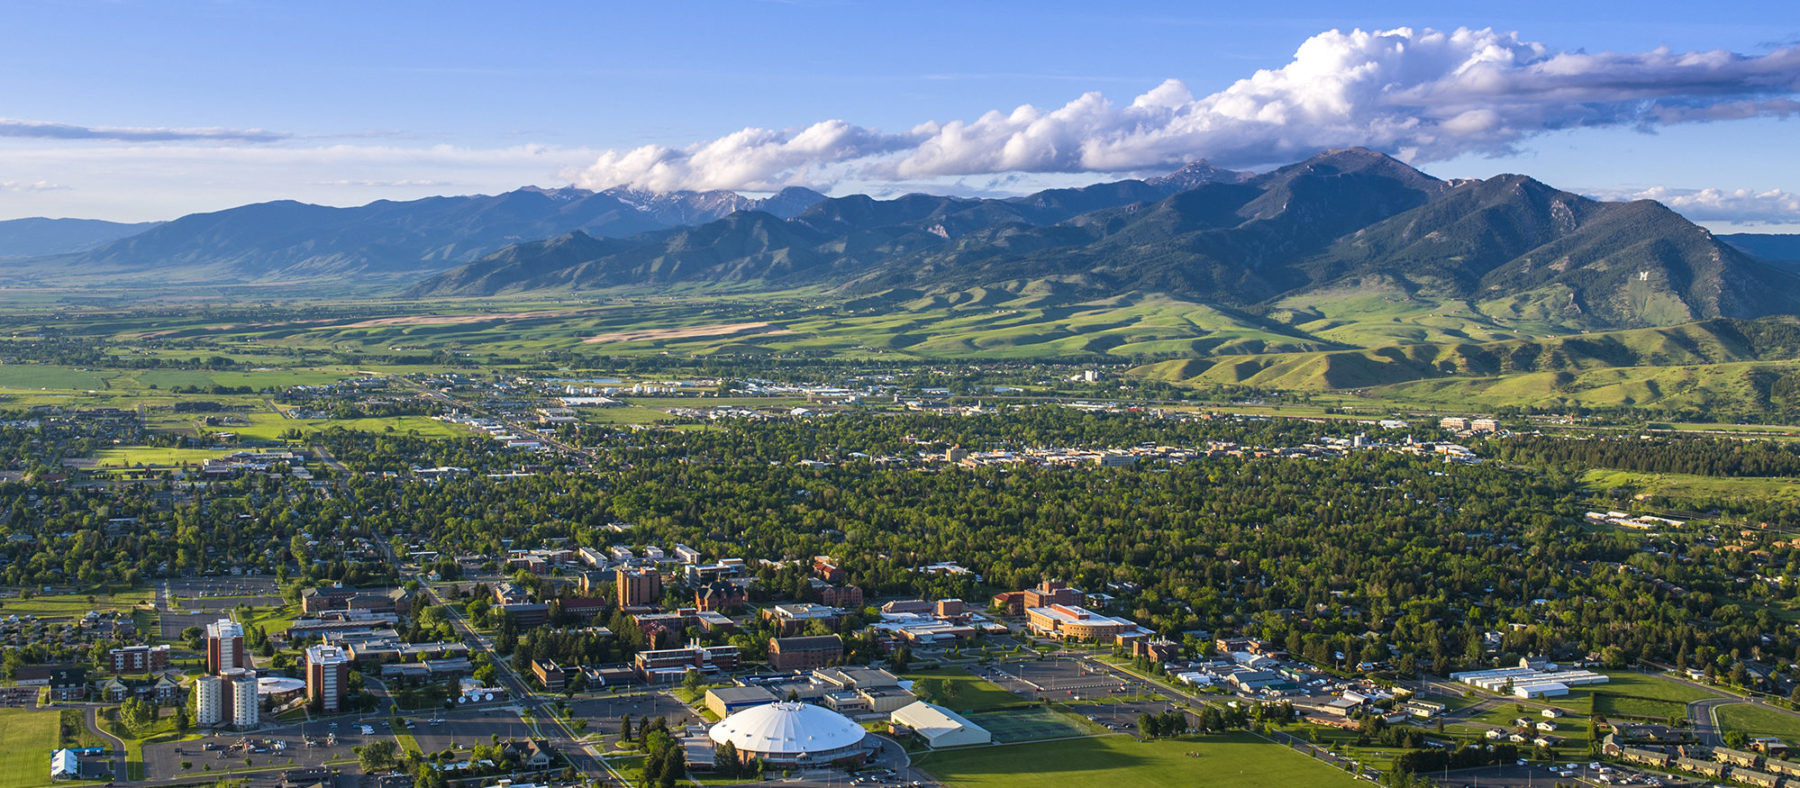
\includegraphics[width=5in,height=\textheight]{images/msu-campus.jpg}
\vspace{1cm}\\
STAT 216 Activity Coursepack}
\usepackage{etoolbox}
\makeatletter
\providecommand{\subtitle}[1]{% add subtitle to \maketitle
  \apptocmd{\@title}{\par {\large #1 \par}}{}{}
}
\makeatother
\subtitle{Spring 2021}
\author{Melinda Yager, Jade Schmidt, Dr.~Stacey Hancock}
\date{}

\begin{document}
\maketitle

\newpage
\thispagestyle{empty}

This resource was developed by Melinda Yager, Jade Schmidt, and Stacey Hancock in 2021 to accompany the online textbook: Carnegie, N., Hancock, S., Meyer, E., Schmidt, J., and Yager, M. (2021). \emph{Montana State Introductory Statistics with R}. Montana State University. \url{https://mtstateintrostats.github.io/IntroStatTextbook/}.

This resource is released under a \href{https://creativecommons.org/licenses/by-nc-sa/4.0/}{Creative Commons BY-NC-SA 4.0} license unless otherwise noted.

\setcounter{tocdepth}{0}
\tableofcontents
\setcounter{page}{1}

\newpage

\hypertarget{preface}{%
\chapter*{Preface}\label{preface}}
\addcontentsline{toc}{chapter}{Preface}

This coursepack accompanies the textbook for STAT 216: Introduction to Statistics at Montana State University. The coursepack includes reading guides to aid in taking notes while you complete the required readings, and in-class activities. Each of the activities in this workbook is designed to target specific learning outcomes of the course, giving you practice with important statistical concepts in a group setting with instructor guidance. Bring this workbook with you to class each week, and take notes in the workbook as you would your own notes. A well-written complete workbook will provide an optimal study guide for exams!

The activities in this coursepack are broken into three sections: pre-class, in-class, and after class. Read through the introduction for each activity and complete the pre-class questions before attending class each week. In class, you will work through the in-class section with your group and instructor. After class, you will complete the out of class part of the activity.

STAT 216 is a 3-credit blended course. Rather than meeting for a total of 150 structured minutes in class per week, students meet with their instructor and cohort of classmates for 50 minutes of class per week. The other 100 minutes typically spent in class are instead spent outside of class watching instructor video lectures, reading the textbook, working through case studies, and participating in online discussion with your classmates. This structure serves two purposes: (1) enhance the safety of our community during the COVID-19 pandemic, and (2) provide additional flexibility for students to create their own schedule and make their own decisions on how they learn best.

In our experience, it takes six to nine hours per week outside of class to achieve a good grade in STAT 216 -- this means six to nine hours outside of the 150 minutes of time set aside for learning course material each week. By ``good'' we mean at least a C because a grade of C- or below does not count toward fulfilling degree requirements. Many of you set your goals higher than just getting a C, and we fully support that. You
need roughly nine hours per week to review past activities, read feedback on previous assignments, complete current assignments, and prepare for the next day's class. A typical week in the life of a STAT 216 student looks like:

\begin{itemize}
\tightlist
\item
  \emph{Prior to weekly class meeting}:

  \begin{itemize}
  \tightlist
  \item
    Read assigned sections of textbook, using the provided reading guides to take notes on the material.
  \item
    Watch assigned videos on that week's content, pausing to take notes and answer video quiz questions.
  \item
    Read through the introduction to the week's in-class activity and complete the pre-class questions.
  \item
    Read through the week's homework assignment and note any questions you may have on the content.
  \end{itemize}
\item
  \emph{In class meeting}:

  \begin{itemize}
  \tightlist
  \item
    Work through in-class activity with your classmates and instructor, taking detailed notes on your answers to each question in the activity.
  \end{itemize}
\item
  \emph{After weekly class meeting}:

  \begin{itemize}
  \tightlist
  \item
    Complete the out-of-class part of the activity, plus any additional parts of the activity you did not complete in class.
  \item
    Review the posted activity solutions and wrap-up videos, and take notes on key points.
  \item
    Finish watching any remaining assigned videos or readings for the week.
  \item
    Read through the week's case study and post case study discussion posts on D2L.
  \item
    Complete the week's homework assignment.
  \end{itemize}
\end{itemize}

\hypertarget{reading-guide-3-introduction-to-r-categorical-data-and-probability}{%
\chapter{\texorpdfstring{Reading Guide 3: Introduction to \texttt{R}, Categorical Data, and Probability}{Reading Guide 3: Introduction to R, Categorical Data, and Probability}}\label{reading-guide-3-introduction-to-r-categorical-data-and-probability}}

\setstretch{1.25}

\hypertarget{section-1.7-data-in-r}{%
\section*{\texorpdfstring{Section 1.7 (Data in \texttt{R})}{Section 1.7 (Data in R)}}\label{section-1.7-data-in-r}}
\addcontentsline{toc}{section}{Section 1.7 (Data in \texttt{R})}

\hypertarget{notes}{%
\subsection*{Notes}\label{notes}}
\addcontentsline{toc}{subsection}{Notes}

\texttt{R} is case sensitive, meaning it reads \texttt{data} differently from \texttt{Data}. If you get an error message, check that your capitalization is correct.

\texttt{R} does not like spaces or special characters This means the column and row headers in the data set should not have spaces, periods, commas, etc. Instead of titling the variable \texttt{column\ header}, use \texttt{column\_header} or \texttt{ColumnHeader}.

\textbf{Tidy data}: Data frames with

\rgi 1 row per \_\_\_\_\_\_\_\_\_\_\_\_\_\_\_\_,

\rgi 1 column per \_\_\_\_\_\_\_\_\_\_\_\_.

We highly recommend completing Tutorial 1 at the end of Chapter 1 (all four lessons) to give you practice with R/RStudio AND to help reflect on the content of Chapter 1: basics of data, sampling, study design, and scope of inference. These tutorials have some content questions and some places for you to practice using R online with some guidance.

\rgi \_\_ indicate spots you need to type in functions, data sets, or variable names.

\rgi There are Hint and Solution buttons on the R code box to help you.

We would not expect you to know the coding right now, especially for things like mutations or creating new variables in the data set. But seeing some initial coding for these more difficult functions will only make you more comfortable using the functions we will use in this course!

\hypertarget{functions}{%
\subsection*{Functions}\label{functions}}
\addcontentsline{toc}{subsection}{Functions}

State what these introductory functions do in \texttt{R}:

\texttt{glimpse(data\_set\_name)}

\texttt{head(data\_set\_name)}

\texttt{data\_set\_name\$variable}

\texttt{\%\textgreater{}\%}

\texttt{\textless{}-}

\hypertarget{section-2.1-exploring-categorical-data}{%
\section*{Section 2.1 (Exploring categorical data)}\label{section-2.1-exploring-categorical-data}}
\addcontentsline{toc}{section}{Section 2.1 (Exploring categorical data)}

\hypertarget{vocabulary}{%
\subsection*{Vocabulary}\label{vocabulary}}
\addcontentsline{toc}{subsection}{Vocabulary}

Frequency table:
\rgs

Relative frequency table:
\rgs

Contingency or Two-way table:
\rgs

Unconditional proportion:
\rgs

Conditional proportion:
\rgs

\rgi Row proportions:
\rgs

\rgi Column proportions:
\rgs

Statistic:
\rgs

\rgi Sample proportion:
\rgs

\rgi \rgi Notation:
\rgs

Parameter:
\rgs

\rgi Population proportion:
\rgs

\rgi \rgi Notation:
\rgs

Bar plot:
\rgs

Segmented bar plot:
\rgs

Simpson's Paradox:
\rgs

\newpage

\hypertarget{notes-1}{%
\subsection*{Notes}\label{notes-1}}
\addcontentsline{toc}{subsection}{Notes}

In a contingency table, which variable (explanatory or response) generally will make the columns of the table? Which variable on the rows?
\rgs

In a segmented bar plot, the bars represent the levels of which variable? The segments represent the levels of which variable?
\rgs

What type of plot(s) are appropriate to display a single categorical variable?
\rgs

What type of plot(s) are appropriate to display two categorical variables?
\rgs

What is the difference between a standardized segmented bar plot and a mosaic plot?
\rgs

True or false: Pie charts are generally highly recommended ways to graphically display categorical data.

True or false: Two categorical variables are associated if the conditional proportions of a particular outcome (typically of the response variable) differ across levels of the other variable (typically the explanatory).

True or false: When a segmented bar plot has segments that sum to 1 (or 100\%), the segment heights correspond to the proportions conditioned on the \textbf{segment}.

\hypertarget{review-of-simpsons-paradox}{%
\subsubsection*{Review of Simpson's Paradox:}\label{review-of-simpsons-paradox}}
\addcontentsline{toc}{subsubsection}{Review of Simpson's Paradox:}

Based on the segmented bar plot in Figure 2.6, which race of defendant was more likely to have the death penalty invoked?
\rgs

Based on the segmented bar plot in Figure 2.7 and Table 2.9, which race of defendant was more likely to have the death penalty invoked when the victim was Caucasian?
\rgs

Based on the segmented bar plot in Figure 2.7 and Table 2.9, which race of defendant was more likely to have the death penalty invoked when the victim was African American?
\rgs

The direction of the relationship between the \_\_\_\_\_\_\_\_\_\_\_\_\_\_
and \_\_\_\_\_\_\_\_\_\_\_\_\_\_ variables is \textbf{reversed} when accounting for
a \_\_\_\_\_\_\_\_\_\_\_\_\_\_ variable.
\rgs

\hypertarget{section-2.2-probability-with-tables}{%
\section*{Section 2.2 (Probability with tables)}\label{section-2.2-probability-with-tables}}
\addcontentsline{toc}{section}{Section 2.2 (Probability with tables)}

\hypertarget{vocabulary-1}{%
\subsection*{Vocabulary}\label{vocabulary-1}}
\addcontentsline{toc}{subsection}{Vocabulary}

Random process:
\rgs

Probability:
\rgs

Hypothetical two-way table:
\rgs

Unconditional probability:
\rgs

\rgi Notation:
\rgs

Conditional probability:
\rgs

\rgi Notation:
\rgs

Event:
\rgs

\rgi Notation:
\rgs

Complement:
\rgs

\rgi Notation:
\rgs

Sensitivity:
\rgs

Specificity:
\rgs

Prevalence:
\rgs

\hypertarget{notes-2}{%
\subsection*{Notes}\label{notes-2}}
\addcontentsline{toc}{subsection}{Notes}

Method for creating a hypothetical two-way table:

\begin{enumerate}
\def\labelenumi{\arabic{enumi}.}
\item
  Start with
  \rgs
\item
  Fill in the column or row totals using
  \rgs
\item
  Fill in the interior cells using
  \rgs
\item
  Add/Subtract to fill in the row/column totals not filled in at step 2.
\end{enumerate}

\rgi \rgi To find unconditional probabilities from the table,
\rgs

\rgi \rgi To find conditional probabilities from the table,
\rgs

\hypertarget{example-baby-jeff}{%
\subsection*{Example: Baby Jeff}\label{example-baby-jeff}}
\addcontentsline{toc}{subsection}{Example: Baby Jeff}

\begin{enumerate}
\def\labelenumi{\arabic{enumi}.}
\item
  Let \(D\) be the event a child has CPK. What does \(D^C\) represent?
  \rgs
\item
  Let \(T\) be the event a child tests positive for CPK. What does \(T^C\) represent?
  \rgs
\item
  Write each of the following values in proper notation:\\
  a. \(1/10000 = 0.0001 = P( \hspace{1in} )\)\\
  b. \(100\% = 1.0 = P( \hspace{1in} )\)\\
  c.~\(99.98\% = 0.9998 = P( \hspace{1in} )\)
\item
  Write out the steps for creating the hypothetical two-way table in section 2.2.4 of your textbook, then copy the table below.
\end{enumerate}

\rgi First,
\rgs

\rgi Next,
\rgs

\rgi After that,
\rgs

\rgi Finally,
\rgs

\rgi Hypothetical two-way table:

\begin{center}
\begin{tabular}{|l|p{1.3in}|p{1.3in}|p{1.3in}|}
\hline
&	Test Positive	& Test Negative	& Total \\ \hline
Has CPK		& & & \\
	& & & \\
	& & & \\ \hline
Does not have CPK		& & & \\
	& & & \\
	& & & \\ \hline		
Total & & & 100,000 \\ \hline
\end{tabular}
\end{center}
\rgs

\begin{enumerate}
\def\labelenumi{\arabic{enumi}.}
\setcounter{enumi}{4}
\item
  What is the probability that a child who had a positive test result actually does have CPK? What notation should be used for this value?
  \rgs
\item
  Explain how the probability in \#5 was calculated.
\end{enumerate}

\end{document}
